\documentclass[10pt,a4paper]{report}

\usepackage[utf8]{inputenc}
\usepackage{amsmath}
\usepackage{amsfonts}
\usepackage{amssymb}
\usepackage{graphicx}
\usepackage{color}
\usepackage{enumitem}
\usepackage[top=1cm, bottom=2cm, left=2cm, right=2cm]{geometry}
\usepackage{hyperref}
\usepackage{fancyhdr}
\pagestyle{fancy}

\fancyhead{}
\fancyfoot{} 
\lhead{ \hspace{0.1cm} M1 WI 2014-2015  \hspace{0.4cm} \vline}
\chead{Apprentissage automatique}
\rhead{K.B - B.B - K.L - N.R}
\rfoot{\thepage}

\author{Kevin BASCOL, Bachir BOUACHERIA, Kevin LAOUSSING, Nicolas REYNAUD}
\title{ Apprentissage automatique : Reconnaissance des formes}

\makeatletter
\renewcommand{\thesection}{\@arabic\c@section}
\makeatother

\begin{document}

\makeatletter
	\begin{titlepage}
	
	\centering
		{
		\vspace*{5cm}
		\hrule height 2pt
		\vspace{0.7cm}
		\Huge \textbf{\@title}}\\
		\vspace{0.7cm}
		\hrule height 2pt
		
		\vfill
		\vspace{1cm}
		\@author\\
		\end{titlepage}
\makeatother
\setcounter{secnumdepth}{4}
\setcounter{tocdepth}{3}
\renewcommand{\contentsname}{Sommaire}
\begingroup\makeatletter
\def\@makeschapterhead#1{%
  {\parindent \z@ \raggedright
    \normalfont
    \interlinepenalty\@M
    \Huge \bfseries  #1\par\nobreak
    \vskip 20pt% <---- à réduire pour avoir plus de place
  }}\makeatother
\tableofcontents
\endgroup
\thispagestyle{empty}
\setcounter{page}{0}
\newpage

\newgeometry{top=2cm, bottom=2cm, left=2cm, right=2cm}

%%%%%%%%%%%%%%%%%%%%%%%%%%%%%%%%%%%%%%%%%%%%%%%%%%%%%%%
%%%					INTRODUCTION					%%%
%%%%%%%%%%%%%%%%%%%%%%%%%%%%%%%%%%%%%%%%%%%%%%%%%%%%%%%
\section{Introduction}
\begin{flushleft}

La reconnaissance de formes est une branche de l'intelligence artificielle qui fait appel aux techniques d'apprentissage de automatique. Durant ce projet, nous avons réalisé un logiciel de reconnaissance de forme, où les formes sont les nombres de 0 à 9.
La réalisation comprend la développement d'une interface graphique ergonomique facilitant la construction d'une base d'apprentissage, la manipulation des algorithmes d'apprentissage et la visualisation des résultats des test d'apprentissage. Et elle comprend aussi l'implémentation de deux méthodes d'apprentissages : les k-plus-proches voisins, et le réseau de neurones.\\
Dans un premier temps nous allons présenter notre organisation autour de ce projet. Puis dans un deuxième temps, nous décrirons les fonctionnalités de notre logiciel. Nous présenterons par la suite les résultats et les performances de notre logiciel à la reconnaissance des nombres.\\
Enfin nous terminerons par une conclusion qui résumera l'efficacité des algorithmes.


\end{flushleft}


%%%%%%%%%%%%%%%%%%%%%%%%%%%%%%%%%%%%%%%%%%%%%%%%%%%%%%%
%%%					ORGANISATION					%%%
%%%%%%%%%%%%%%%%%%%%%%%%%%%%%%%%%%%%%%%%%%%%%%%%%%%%%%%

\section{Organisation du projet}

\subsection{Planning}

\paragraph{planning au prévisionnel }
\begin{flushleft}
•
\end{flushleft}



%%%%%%%%%%%%%%%%%%%%%%%%%%%%%%%%%%%%%%%%%%%%%%%%%%%%%%%
%%%					FONCTIONNALITES				%%%
%%%%%%%%%%%%%%%%%%%%%%%%%%%%%%%%%%%%%%%%%%%%%%%%%%%%%%%

\section{Fonctionnalités}

\subsection{Interface graphique}
\begin{figure}[!h]
	\center
		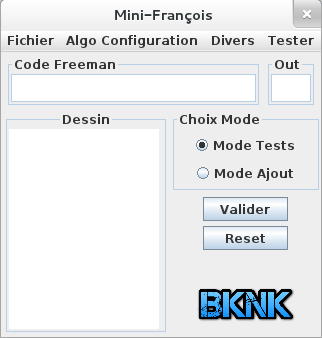
\includegraphics[scale=0.5]{./Ressource/IG.png}
 	\caption{Interface graphique de Mini-François}
\end{figure}
\subsubsection{Module de saisi de données}
\begin{flushleft}
Pour interagir avec le logiciel nous avons développé un module de saisi possédant deux modes : un mode permettant de générer des données d'apprentissage pour créer une base d'apprentissage, et un mode pour tester notre système.\newline
Le module est composé de :

\begin{itemize}
\item un cavena de dimension de 200x150 pour dessiner un chiffre à la souris.

\item un champ de texte "out/in" dans lequel on indique le chiffre qu'on dessine dans le cavena.

\item un autre champ de texte "code de freeman" dans lequel apparaît le code freeman du chiffre dessiné.

\item un groupe de deux radio-boutons pour sélectionner le mode du module de saisi.

\item un bouton "Valider" pour valider l'acquisition de la donnée (en mode ajout) et pour lancer le test (en mode test).

\item un bouton "Reset" pour annuler l'acquisition de la donnée en cas d'erreur. (Par exemple si on dessine un chiffre A dans le cavena mais qu'il ne correspond pas au chiffre B entré dans le champ de texte "out/in" et qu'on a valider l'acquisition par mégarde, il est possible d'annuler l'acquisition grâce au bouton "Reset").
\end{itemize}

\end{flushleft}

\begin{figure}[!h]
	\center
		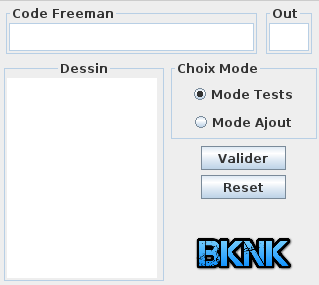
\includegraphics[scale=0.5]{./Ressource/Module_saisi.png}
 	\caption{Module de saisi de données}
\end{figure}

\paragraph*{Mode test}
\begin{flushleft}
Si le radio bouton "Mode Test" est sélectionné alors le logiciel lance l'algorithme avec les paramètres spécifiés dans le menu "Algo configuration" et le chiffre dessiné dans le cavena.
\end{flushleft}


\paragraph*{Mode ajout}
\begin{flushleft}
Si le radio bouton "Mode Ajout" est sélectionné alors le logiciel enregistre le code de freeman et la matrice correspondant au chiffre dessiné dans le cavena dans un fichier "Base" correspondant à la base d'apprentissage du logiciel.
\end{flushleft}

\subsubsection{Module de configuration}

\begin{flushleft}
Le module de configuration permet de renseigner les paramètres de nos algorithmes. Il est accessible à partir du menu "Algo Configuration".\\
On peut cocher l'algorithme (ainsi que les paramètres qu'on souhaite utiliser") que le logiciel doit utiliser en "mode test". 
\end{flushleft}

\subsubsection{Module de visualisation statistique des données d'apprentissages}
\begin{flushleft}

\end{flushleft}

\subsection{Algorithmes d'apprentissage}

\subsubsection{Base d'apprentissage}

\subsubsection{Algorithme k-PPV}
l'utilisation de l'algorithme des k plus proches voisins, consiste à résoudre la problématique en utilisant des distances.
dans notre application, on a utilisé 4 distances différentes qui sont : Distance euclidienne
- Distance de Manhattan 
- Distance de Chebyshev
- Distance d'édition(où de Levenshtein)
tel-que l'algorithme utilise les 3 premières distances pour comparer des matrices entre elles, alors que la distance d'édition est utilisés pour trouver la distance entre deux chaine de code de Freeman 
qui représentent le chiffre.
Après plusieurs essayes, on a constaté que l'algorithme des k plus proche voisin est plus performant quand on utilise la distance d'édition (code de Freeman), contrairement à l'utilisation de la distance de Chebyshev.
quant à l'utilisation de nombre différent de voisins (3-ppv, 5-ppv et 7-ppv), on constate qu'il n'y a pas une grande différence entre les taux de réussite.
\subsubsection{Algorithme réseau de neurones}
\begin{flushleft}

Pour le réseau de neurones, comme nous étions en retard, nous avons choisi d'utiliser une implémentation déjà faite sur internet. Nous avons choisit d'utiliser celle de WEKA comme nous avions déjà eu un apperçu pendant la séance de TP.\\
\vspace*{0.3cm}
Tout d'abord nous avons tenté d'utiliser comme entrée la matrice. Comme nous utilisons une matrice de 150x200 celle-ci donnerait un nombre trop conséquent de pixel à passer en entrée. Nous avons donc réduit la matrice à l'aide d'une matrice 10x10 ce qui a réduit le nombre d'entrée à 300.

\end{flushleft}


%%%%%%%%%%%%%%%%%%%%%%%%%%%%%%%%%%%%%%%%%%%%%%%%%%%%%%%
%%%						ETUDE						%%%
%%%%%%%%%%%%%%%%%%%%%%%%%%%%%%%%%%%%%%%%%%%%%%%%%%%%%%%

\section{Etude}

\subsection{Description de la fonctionnalité}
\begin{flushleft}
•
\end{flushleft}

\subsection{Description technique}
\begin{flushleft}
•
\end{flushleft}


%%%%%%%%%%%%%%%%%%%%%%%%%%%%%%%%%%%%%%%%%%%%%%%%%%%%%%%
%%%						CONCLUSION					%%%
%%%%%%%%%%%%%%%%%%%%%%%%%%%%%%%%%%%%%%%%%%%%%%%%%%%%%%%

\section{Conclusion}
\begin{flushleft}
•
\end{flushleft}


%%%%%%%%%%%%%%%%%%%%%%%%%%%%%%%%%%%%%%%%%%%%%%%%%%%%%%%
%%%						ANNEXES						%%%
%%%%%%%%%%%%%%%%%%%%%%%%%%%%%%%%%%%%%%%%%%%%%%%%%%%%%%%

\section{Sources}
\begin{description}
	\item[WEKA] \url{http://weka.sourceforge.net/doc.dev/overview-summary.html}
\end{description}
\end{document}
